\section{Hintergrund}
In diesem Kapitel wird auf die Konzepte und Begriffe von Webcrawlern und Machine Learning eingegangen. Es soll ein gemeinsames Grundwissen für beide Gebiete geschaffen werden.
%
\subsection{Webcrawler}
Um Informationen von Webseiten zu sammeln, muss deren Inhalt analysiert und die gewünschten Daten extrahiert werden. Für diese Aufgabe eignen sich Webcrawler besonders gut \cite{scrapy_1, scrapy_2}.\\
Dabei erhält ein Webcrawler eine oder mehrere Einstiegs-URLs. Diese werden dann vom Crawler aufgerufen und die dazugehörigen Seiten ausgewertet. Bei der Auswertung kann der Crawler auf weitere URLs stossen, die er in seine Liste der abzuarbeitenden URLs aufnehmen kann. Sind alle URLs abgearbeitet, ist der Crawler fertig. Je nach Aufgabenbereich existieren verschiedene Crawler-Techniken.\\
Ist bekannt von welchen Seiten die Informationen gecrawlt werden können, eignet sich am besten ein fokussierter Crawler. Dieser Crawler steuert vordefinierte Seiten an und extrahiert Informationen nach vorgegebenen Regeln.\\
Sind die Webseiten nicht bekannt oder haben die gesuchten Informationen keine definierte Struktur, eignen sich Deep Web Crawler. Diese bewegen sich mehrheitlich autonom und versuchen durch analysieren des Inhaltes herauszufinden, ob der Inhalt von Interesse ist oder nicht.\\
Sind übermässig viele Seiten zu crawlen, oder ist die Stabilität der Crawler wichtig, kommen verteilte Crawler zum Einsatz. Durch die Verteilung wird an Stabilität gewonnen und die Last auf die verschiedenen Crawler verteilt \cite{scrapy_3}.\\[2ex]
%
Um Daten von einer Webseite zu extrahieren, gibt es diverse Möglichkeiten. Von der einfachen String-Suche bis zu Machine Learning Methoden kann nahezu alles angewandt werden. Beim fokussierten Crawlen wird häufig versucht Informationen über den XPATH oder über die CSS-Klassen zu extrahieren. Beide Varianten haben ihre Vor- und Nachteile, sind aber im Grunde sehr ähnlich \cite{xpath_vs_css}. Somit ist es dem Benutzer überlassen, welche Variante er wählt \cite{xpath}.\\[2ex]
%
Eine Herausforderung beim Crawlen ist, dass der Crawler nicht als solchen vom Webseitenbetreiber erkannt wird. Diverse Betreiber möchten gerne verhindern, dass Informationen von Ihren Seiten gecrawlt werden \cite{comparis}.\\
Ist ein Crawler zu aggressiv, kann es vorkommen, dass er vom Betreiber gesperrt wird. Es gilt daher mit einer gewissen Raffinesse vorzugehen. Um möglichst nicht aufzufallen, ist es sinnvoll nur ein paar Requests\footnote{Anfrage auf eine Webseite} pro Minute abzusetzen und einen existierenden User Agent String\footnote{Browser Kennung für die Webseite} anzugeben. Wenn das nicht ausreichend ist, können die Seiten über einen Pool von rotierenden IP-Adressen aufgerufen werden. So ist die Quelladresse nicht immer dieselbe \cite{offensive_crawling}.
%
\subsection{Machine Learning}
Machine Learning ist eine Art Künstliche Intelligenz (KI), das Softwareapplikationen erlaubt Vorhersagen anhand von trainierten Algorithmen zu erstellen.
Die Definition von Machine Learning aus dem Jahr 1959 von Arthur Samuel, einer der Pioniere im Bereich Machine Learning, lautet \cite{what_is_ml}:
  \begin{quote}
  \textit{Machine Learning: Field of study that gives computers the ability to learn without being explicitly programmed.}
  \end{quote}
Mit Hilfe von Machine Learning Algorithmen können neben Vorhersagen auch Trends erkannt oder Klassifizierungen durchgeführt werden \cite{ml_book}.
Dabei handelt es sich nicht um eine exakte Wissenschaft. Es lohnt sich verschiedene Algorithmen mit unterschiedlichen Parametern auszuprobieren, um die beste Performance zu finden. Vieles hängt auch von den Ausgangsdaten ab \cite{ml_azure}.

Grundsätzlich erhält ein Algorithmus Daten, die er zu einem Modell verarbeitet. Dieses Modell wird ausgewertet. Entspricht es nicht den gewünschten Anforderungen wird versucht ein besseres Modell zu erstellen, bis das Resultat zufriedenstellend ist. Abbildung \ref{fig:ml_process} zeigt den schematischen Ablauf.\\
\begin{figure}[ht]
\centering
\begin{tikzpicture}[
  font=\sffamily,
  every matrix/.style={ampersand replacement=\&,column sep=1.5cm,row sep=.5cm},
  source/.style={draw,thick,rounded corners,fill=yellow!20,inner sep=.3cm},
  process2/.style={draw,thick,rounded corners,fill=blue!20,inner sep=.3cm},
  process/.style={draw,thick,circle,fill=orange!20},
  process3/.style={draw,thick,rounded corners,fill=orange!20, inner sep=.3cm},
  sink/.style={source,fill=green!20},
  datastore/.style={draw,very thick,shape=datastore,inner sep=.3cm},
  dots/.style={gray,scale=2},
  to/.style={->,>=stealth',shorten >=1pt,semithick,font=\sffamily\footnotesize},
  dotted/.style={dashed,->,>=stealth',shorten >=1pt,semithick,font=\sffamily\footnotesize},
  every node/.style={align=center}]
% Position the nodes using a matrix layout
\matrix{
  \node[source] (data) {Data};
      \& \node[process] (model) {Model};
        \& \node[sink] (prediction) {Prediction}; \\
};

% Draw the arrows between the nodes and label them.
\draw[to] (data) -- node[midway,above] {Train}
    node[midway,below] {} (model);

\draw[to] (model) -- node[midway,above] {Predict}
    node[midway,below] {} (prediction);

\draw[to] (prediction) to[bend right=50] node[midway,above] {Evaluate}
    node[midway,below] {} (data);
\end{tikzpicture}
\caption[Schematischer Ablauf bei Machine Learning]{Schematischer Ablauf bei Machine Learning}%
\label{fig:ml_process}
\end{figure}

\begin{samepage}
Machine Learning Algorithmen lassen sich grob in die folgenden Kategorien einteilen \cite{super_unsuper}:
\begin{description}
  \item[Supervised Learning]	Bei diesen Algorithmen sind die Daten gekennzeichnet. Das heisst, es ist erkenntlich, welchen Beobachtungswert die Daten darstellen. Mit Hilfe dieser Daten, wird ein Modell erstellt, das möglichst nahe den Beobachtungswert schätzt. Dabei kann es sich um eine Klassifizierung oder Regression handeln.
  \item[Unsupervised Learning] Hier sind die Daten nicht gekennzeichnet. Es wird versucht Muster zu erkennen. Anhand von diesen Mustern können unter anderem Trends oder Ausreisser erkannt werden.
  \item[Reinforcement Learning] Hier lernt der Algorithmus anhand seiner Aktionen. Für jede Aktion, die er berechnet, wird er entweder belohnt oder bestraft. Mit genug Iterationen kann der Algorithmus situationsbedingte Abläufe erlernen und später anwenden.
\end{description}
\end{samepage}

Für eine Schätzung braucht jeder Machine Learning Algorithmus ein berechnetes Modell. Dieses kann unter anderem eine mathematische Formel oder eine Baumstruktur sein. Damit ein Modell erstellt werden kann, braucht jeder Algorithmus ein oder mehrere Features. Features sind messbare Merkmale, die einen Beobachtungswert, auch Target genannt, beschreiben. Es ist sinnvoll die Features im Voraus zu untersuchen und herauszufinden, welche Features wichtig sind und welche weggelassen werden können. Dabei können auch Features miteinander kombiniert werden. Dieses Vorgehen wird Feature Engineering genannt.\\[2ex]
%
Damit ein Algorithmus überprüfen kann, wie gut seine Schätzungen sind, wird der Fehler, beziehungsweise die Residuen berechnet. Die Differenz zwischen einem geschätztem Wert und dem dazugehörigen beobachteten Wert wird als Residuum bezeichnet. Es sind systematische\footnote{Ein falsches Modell wurde verwendet.} wie auch statistische Fehler\footnote{Es handelt sich um Ausreisser.} im Residuum mit eingerechnet. Formel \eqref{eq:residuals} zeigt die Berechnung der Residuen, dabei ist $\hat{y}$ der geschätzte Wert und $y$ der beobachtete Wert.

\begin{equation}
\label{eq:residuals}
\hat{\varepsilon} = y - \hat{y}
\end{equation}

\begin{table}[h]
\centering
\ra{1.3}
\resizebox{\textwidth}{!}{
\begin{tabular}{@{}llll@{}}
\toprule
Name & Abkürzung & Formel & Modellart\\
\midrule
Mean Absolute Error & MAE & $\frac1n \sum_{i=1}^{n} |y_i - \hat{y_i}|$ & absolut\\
Median Absolute Error & MdAE & $med(\sum_{i=1}^{n} |y_i - \hat{y_i}|)$ & absolut\\
Sum of Squared Errors & SSE & $\sum_{i=1}^{n} (y_i - \hat{y_i})^2$ & quadratisch\\
Root Mean Squared Errors & RMSE & $\sqrt{\frac1n \sum_{i=1}^{n} (y_i - \hat{y_i})^2}$ & quadratisch\\
Mean Absolute Percentage Error & MAPE & $\frac1n \sum_{i=1}^{n} |\frac{y_i - \hat{y_i}}{y_i}|, y_i \neq 0$ & prozentual\\
Median Absolute Percentage Error & MdAPE & $med(\sum_{i=1}^{n} |\frac{y_i - \hat{y_i}}{y_i}|), y_i \neq 0$ & prozentual\\
\bottomrule
\end{tabular}}
\caption{Fehlermodelle mit Formeln}
\label{tab:error_models}
\end{table}

Wie in Tabelle \ref{tab:error_models} gezeigt, haben sich mit der Zeit diverse Fehlermodelle entwickelt \cite{error_models}. Die Wahl des Fehlermodells ist vom Anwendungsfall abhängig. Grundsätzlich können Fehler absolut, quadratisch oder prozentual berechnet werden.\\
Bei absoluten Werten werden alle Fehler gleich stark gewichtet, wobei beim quadratischen Fehlermodell grössere Fehler durch Quadrieren stärker gewichtet werden. Beim MAE hat ein Fehler bei einem hohen Beobachtungswert einen grösseren Einfluss auf den gesamten Fehler. Das kann durch den Median (MdAE) oder einer prozentualen Angabe wie der MAPE oder MdAPE vermieden werden. Eine prozentuale Angabe hat zusätzlich den Vorteil, dass sie intuitiver interpretiert werden kann. Der Nachteil bei MAPE und MdAPE ist, dass sie bei einem $y$ Wert von 0 nicht verwendet werden können \cite{error_models_2}.

Eine weitere Möglichkeit die Performance eines Modells neben dem Fehlermodell zu bestimmen, ist der $R^2$ Wert. $R^2$ ist ein Gütemass, das beschreibt, wie gut die Features in der Lage sind, die Varianz der Zielvariable erklären zu können. Dabei ist $y$ der Beobachtungswert, $\hat{y}$ der geschätzte Wert und $\overline{y}$ der Durchschnitt aller gegebenen $y$. Sind alle Beobachtungswerte gleich, ist $R^2$ nicht definiert. Die Interpretation der Formel \eqref{eq:r2} zeigt, dass mit einem hohen Wert (maximal 1) die statistische Varianz der Daten gut erklärt werden kann. Mit einem tiefen Wert (gegen 0), kann die Varianz nicht gut erklärt werden. \\
Es gilt jedoch zu beachten, dass der $R^2$ Wert die Varianzen aufzeigt. Somit kann nicht davon ausgegangen werden, dass ein hoher $R^2$ Wert auch eine hohe Genauigkeit beim Schätzen erzielt \cite{r2, r2_2}.

\begin{equation}\label{eq:r2}
R^2 = 1 - \frac{\sum_{i=1}^{n} (y_i - \hat{y_i})^2}{\sum_{i=1}^{n}(y_i - \overline{y})^2},\text{ falls } \neg \forall y:y = \overline{y}
\end{equation}

Es macht keinen Sinn auf denselben Daten zu trainieren und das Modell zu überprüfen. Deshalb wird der Datensatz in mindestens einen Trainings- und einen Testdatensatz aufgeteilt \cite{cross_validation}.
Dadurch kann die Gefahr eines Overfits\footnote{Überanpassung} verringert werden. Bei einem Overfit wurde das Modell zu stark an den Trainingsdaten trainiert und schneidet bei den Testdaten schlecht ab. Wichtig dabei ist, dass die Daten vor dem Aufteilen gut gemischt werden. So soll beispielsweise verhindert werden, dass nicht nur Wohnungen im Trainings\-datensatz und nicht alle Häuser nur im Testdatensatz sind.\\
Cross Validation ist eine weitere Möglichkeit den Datensatz aufzuteilen. Dieser teilt den gesamten Datensatz in K-Teile auf. Dabei werden K-1 Datensätze für das Trainieren und 1 Datensatz für das Testen verwendet. Das Ganze wird K-mal wiederholt, so dass jeder Datensatz einmal als Testdatensatz verwendet wird.
%
\subsubsection{Lineare Regression}
Bei der Linearen Regression wird versucht, anhand einer linearen Funktion einen Beobachtungswert $y$ durch einen oder mehrere Features aus $X$ zu berechnen. Dabei handelt es sich um ein statistisches Verfahren, bei dem davon ausgegangen wird, dass $y$ abhängig von $X$ ist. Weiter gilt, dass die unabhängigen Variablen $X$ dichotom oder intervallskaliert sind.

\begin{equation}\label{eq:linear}
\hat{y} = h_\theta(x) = \sum_{j=0}^{N} \theta_j x_j
\end{equation}

Formel \eqref{eq:linear} zeigt die lineare Regression wobei $\theta$ den Koeffizienten für jedes einzelne Feature darstellt. Je höher der Koeffizient ist, desto mehr Gewicht hat dieses Feature im Modell. Um auf die optimalen Koeffizienten zu kommen, versucht der Algorithmus eine Gerade durch den Datensatz zu ziehen, die zu allen Punkten den kleinstmöglichen Abstand hat. Der Algorithmus versucht folglich, das Schätzungsmodell auf das gewählte Fehlermodell zu optimieren. Zugleich dient das Fehlermodell auch als Performancemetrik. Die Optimierung wird durch die Kostenfunktion \eqref{eq:cost_function} berechnet. Oft wird dafür die \textit{Ordinary Least Squares} (OLS) Methode genommen. Wird auf diesem Algorithmus optimiert, können auch andere, spezifischere Kostenfunktionen eingesetzt werden.

\begin{equation}\label{eq:cost_function}
J(\theta) = \frac{1}{2m} \sum_{i=1}^{N} (h_\theta(x^i) - y^i)^2
\end{equation}

Das quadratische Fehlermodell macht den Algorithmus anfälliger auf Ausreisser. Diese sollten, wenn immer möglich, in einem vorherigen Schritt erkannt und herausgefiltert werden. Auch sollte der Fehler in den Daten normalverteilt sein und die Residuen eine Homoskedastizität aufweisen, da ansonsten keine gute Regression gefunden wird \cite{gradient_descent, gradient_descent_2, gradient_descent_3}.

\textbf{Polynomial Regression}\\
In vielen Fällen hat der Datensatz keine Homoskedastizität, sondern besitzt eine Heteroskedastizität \cite{poly}. Dies ist oft dann der Fall, wenn das Verhältnis zwischen y und X einer Kurve entspricht. In solch einem Fall erzielt die lineare Regression keine gute Performance.
Bei der Polynomialen Regression ist deshalb das beste Modell keine Gerade durch den Datensatz, sondern ähnelt der einer Kurve. Je mehr Polynome die Regression besitzt, desto kurvenreicher ist die Funktion am Schluss. Die Formel für eine Polynomgleichung zweiten Grades wird in Gleichung \eqref{eq:poly} dargestellt.

\begin{equation}\label{eq:poly}
y = \theta_0 + \theta_1 * X + \theta_2 * X^2
\end{equation}

Je höher der Grad des Polynoms, desto genauer wird der Algorithmus auf den Trainingsdatensatz trainiert. Das hat den Nachteil, dass neue Datensätze ungenau geschätzt werden, da das Modell eine hohe Varianz aufweist. Dieses Phänomen nennt sich Overfitting. Der Algorithmus wurde somit zu stark am Trainingsdatensatz trainiert.\\
Ist der Grad des Polynoms zu klein gewählt, kommt es zu einem Underfitting. Das Modell kann nur Features abbilden, die dem ausgewählten Grad entsprechen. Alle anderen Features werden ignoriert. So entsteht die Gefahr, dass wichtige Features nicht ins Modell mit einfliessen und das Modell ein hohes Bias besitzt. Abbildung \ref{fig:under_overfit} zeigt den Vergleich von Underfit zu einem Overfit.\\
Es wird auch vom \textit{Bias-Varianz-Dilemma} gesprochen \cite{bias_variance, bias_variance_2}. Die Kunst ist, die richtige Abstimmung zu finden, damit das Modell die beste Performance hat.

\begin{figure}[ht]
\centering
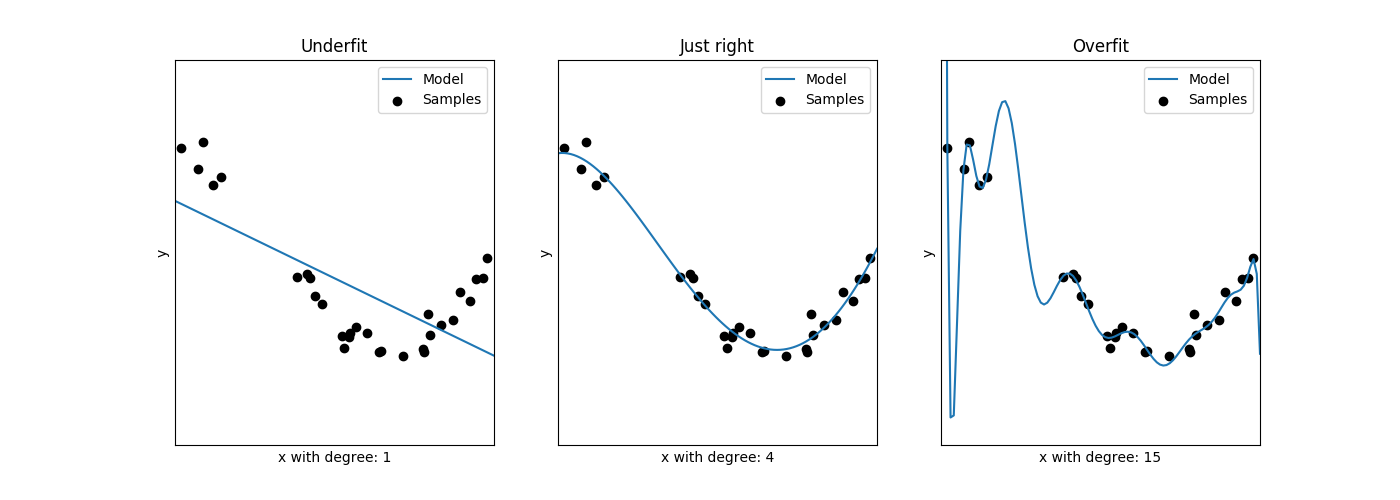
\includegraphics[width=\textwidth]{images/overfit_underfit.png}
\caption[Vergleich von Overfit zu Underfit]{Vergleich von Overfit zu Underfit}
\label{fig:under_overfit}
\end{figure}

Das Bias-Varianz-Dilemma ergibt sich durch die Komplexität eines Modells. Die Komplexität wird durch Hinzufügen von Polynomen oder Features gesteigert.
Es ist daher sinnvoll die Modelle möglichst einfach zu gestalten oder einen Regularisierungsparameter zu verwenden.

\textbf{Ridge Regression}\\
Ridge Regression ist ein Linearer Regression Algorithmus mit einem Regularisierungsparameter $\lambda$. Anhand von diesem kann der Algorithmus die Koeffizienten der einzelnen Features verkleinern und somit die Komplexität reduzieren. Infolgedessen wird $\lambda$ auch Schrumpfparameter genannt. Je höher dieser gewählt wird, desto schwächer werden die Koeffizienten \cite{ridge, ridge_2}. Formel \eqref{eq:ridge} zeigt die Definition von Ridge Regression.

\begin{equation}
\label{eq:ridge}
J(\theta) = \frac{1}{2m} \sum_{i=1}^{N} (h_\theta(x^i) - y^i)^2 + \lambda \sum_{j=0}^{M} \theta_{j}^{2}
\end{equation}

Wichtig beim Ridge Algorithmus ist, dass die einzelnen Koeffizienten verkleinert werden, aber nie 0 erreichen. Das geeignetste Lambda hängt immer vom Datensatz ab und muss durch analysieren verschiedener Werte gefunden werden.

\textbf{Lasso Regression}\\
Ein weiterer Regularisierungsalgorithmus ist der Lasso Regression Algorithmus \eqref{eq:lasso}. Dieser fügt, wie der Ridge Regression auch, einen zusätzlichen $\lambda$ Parameter ein. Er nimmt dabei nicht das $\theta$ im Quadrat, sondern den absoluten Wert von $\theta$ und summiert diesen auf. Durch das kann der Algorithmus unwichtige Features auf 0 setzen und eliminieren. Wenn Features weggelassen werden, wird die Komplexität des Modells reduziert \cite{lasso}.

\begin{equation}\label{eq:lasso}
J(\theta) = \frac{1}{2m} \sum_{i=1}^{N} (h_\theta(x^i) - y^i)^2 + \lambda \sum_{j=0}^{M} |\theta_j|
\end{equation}

\subsubsection{$K$-Nearest Neighbor}
Der $K$-Nearest Neighbor Algorithmus (KNN) ist ein unsupervised Algorithmus und kann für Klassifizierungs- wie auch für Regressionsmodelle verwendet werden. In dieser Arbeit wird er als Regressionsmodell verwendet.\\
Der KNN-Algorithmus sucht für einen Datensatz die $K$ ähnlichsten Datensätze aus dem Trainingsset. Als Schätzung gibt er den Durchschnitt der gefundenen Werten an \cite{knn_1}. KNN ist folgendermassen definiert \eqref{eq:knn_1}:

\begin{equation}\label{eq:knn_1}
\hat{y} = \frac{1}{K} \sum_{i=1}^{K} (y_{knj})
\end{equation}

Wobei $\hat{y}$ der geschätzte Wert darstellt, $K$ die Anzahl Datensätze, die für die Schätzung einbezogen werden und $y_{knj}$ die gefundenen Beobachtungswerte, die am nächsten zum gesuchten Punkt liegen.\\
Die Distanzberechnung von einem gesuchten Punkt kann mit unterschiedlichen Algorithmen berechnet werden. Häufig wird der Euklid, wie in Formel~\eqref{eq:euklid} gezeigt, verwendet, da er alle Dimensionen gleichbehandelt. Wie beim quadratischen Fehlermodell, ist auch der Euklid anfällig auf grosse Ausreisser. Um das zu verhindern, kann der Manhattan oder Chebyshev Algorithmus verwendet werden. Beim Manhattan Algorithmus werden Querdistanzen höher gewichtet als gerade Distanzen. Im Gegensatz zum Chebyshev Algorithmus, bei dem alle Richtungen gleich gewichtet werden.

\begin{equation}\label{eq:euklid}
D(x, p_i) = \sqrt{(x - p_i)^2}
\end{equation}

Auch bei diesem Algorithmus tritt die Gefahr von einem Underfit und Overfit auf. Wird $K$ zu gross gewählt, kommt es zu einem Underfit. Ist $K$ sehr klein, kann es zu einem Overfit kommen. Das optimale $K$ hängt vom Datensatz und der gewünschten Performance ab. Abbildung \ref{fig:under_overfit_knn} zeigt den Vergleich von einem Underfit zu einem Overfit bei einem KNN Algorithmus.

\begin{figure}[ht]
\centering
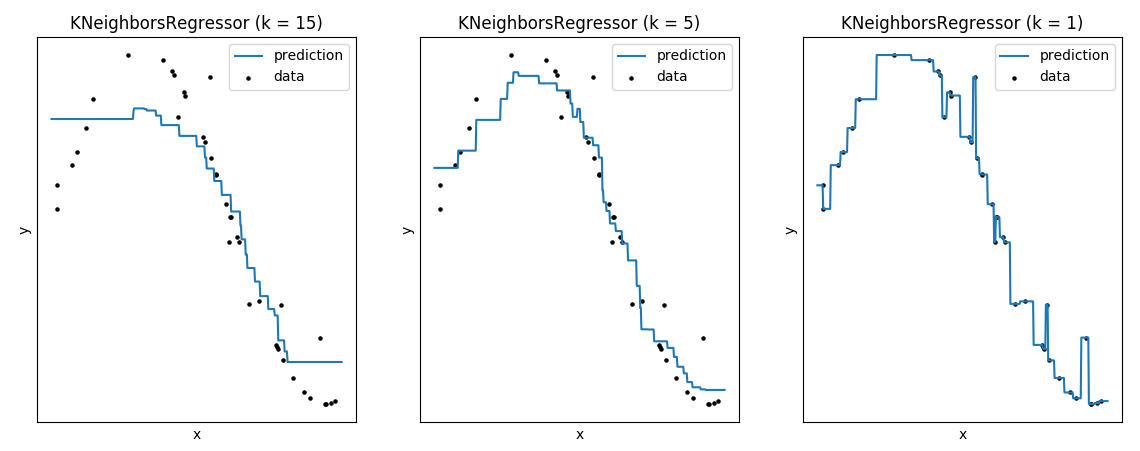
\includegraphics[width=\textwidth]{images/knears_overfit.png}
\caption[Vergleich von Overfit zu Underfit bei einem KNN]{Vergleich von Overfit zu Underfit bei einem KNN}
\label{fig:under_overfit_knn}
\end{figure}

Der KNN Algorithmus kann erweitert werden, indem näher gelegene Punkte stärker gewichtet werden als weiter entfernte. So ist der Algorithmus weniger anfällig auf unregelmässige Daten oder Ausreisser.\\
Für die Gewichtung eines Punktes wird folgende Formel verwendet~\eqref{eq:knn_weights}:

\begin{equation}
\label{eq:knn_weights}
W(x, p_i) = \frac{e^{(-D(x, p_i))}}{\sum_{i=1}^{K} e(-D(x, p_i))}
\end{equation}

$D(x, p_i)$ ist die Distanz vom gesuchten Punkt $x$ zum nächsten Punkt $i$ im Trainingsset. Da immer durch die Summe aller Distanzen dividiert wird, ist der Wert immer zwischen 0 und 1. Näher gelegene Punkte erhalten somit eine höhere Gewichtung $W$. Die Summe aller Gewichte ergibt immer 1.\\
Die Gewichtung wird mit dem gefundenen Beobachtungswert multipliziert, wie in Formel \eqref{eq:knn_with_weights} gezeigt. Die Durchschnittsberechnung muss nicht durchgeführt werden, da die Gewichtung normalisierte Werte zurückgibt \cite{knn_2, knn_3}.

\begin{equation}
\label{eq:knn_with_weights}
\hat{y} = \sum_{j=1}^{K} W(x_0, x_i) y_i
\end{equation}

\subsubsection{Baum Algorithmen}
Ein anderer Ansatz von Machine Learning besteht aus den Tree Based Learning Algorithmen. Am verbreitetsten sind Classification and Regression Trees (CART), die von Breiman 1984 beschrieben wurden. Darunter gibt es noch diverse ähnliche Algorithmen\footnote{ID3, C4.5, CHADI, MARS, Conditional Inference Trees}. Bei diesen Algorithmen handelt es sich grundsätzlich um supervised Algorithmen. Es existieren aber auch unsupervised Ansätze, die nicht Teil dieser Arbeit sind.

\textbf{Decision Trees}

\begin{figure}[h]\label{fig:decision_tree}
  \centering
  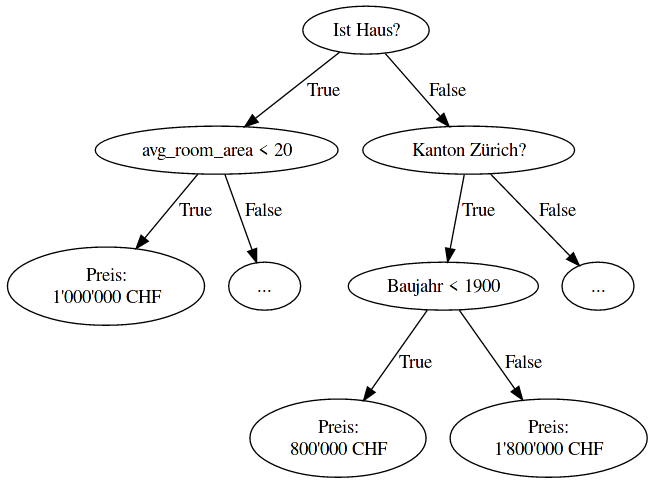
\includegraphics[width=0.7\textwidth]{images/decision_tree.png}
  \caption[Aufbau eines Entscheidungsbaumes]{Aufbau eines Entscheidungsbaumes}
\end{figure}

Ein Decision Tree\footnote{Entscheidungsbaum} ist eine Baumstruktur, die es erlaubt, Daten mithilfe von Entscheidungsregeln zu kategorisieren. Bei den Daten kann es sich sowohl um diskrete als auch um kontinuierliche Werte handeln.\\
Auf jedem Knoten des Entscheidungsbaumes wird ein Feature aus dem Datensatz ausgewählt und eine Teilung in seinem Wertebereich durchgeführt. Der Feature Raum wird somit in unterschiedliche, nicht überlappende Regionen aufgeteilt. Es gilt zu beachten, dass dasselbe Feature wiederholt als Entscheidungsregel verwendet werden kann.

Für eine Schätzung wird der Durchschnitt aller Werte in den Regionen $R_j$ berechnet, in die der zu schätzende Wert fällt.\\
Wie die  $J$ unterschiedliche Regionen aufgeteilt werden, hängt von der Kostenfunktion ab. Bei der Regression wird dafür der Residual Sum of Squares (RSS) verwendet. Das Ziel ist es, die Regionen $R_1$, $R_2$ … $R_j$ so zu legen, dass der RSS minimiert wird. Das kann anhand der Formel \eqref{eq:decision_tree} erreicht werden.

\begin{equation}
\label{eq:decision_tree}
\sum_{j=1}^{J} \sum_{j \in R_j}^{} (y_i - \hat{y}_{R_j})^2
\end{equation}

Dabei ist $\hat{y}_{R_j}$ der durchschnittliche Beobachtungswert in der $j$-ten Region. Für eine Klassifikation werden andere Kostenfunktionen wie der Gini Coefficent oder Gini Impurity verwendet.

Da es aber mit steigender Anzahl von Datensätzen praktisch unmöglich wird, jede mögliche optimale Region durchzurechnen, wird ein “greedy” Ansatz verwendet. Greedy deshalb, weil die nächstbeste Teilung nur mit den aktuell vorhandenen Regionen berechnet wird. Es wird nicht rekursiv vorausberechnet um mit weiteren Teilungen ein theoretisch besserer Baum zu erstellen. So wird nur ein lokales und kein globales Optimum gefunden. Die Aufteilung einer Region in zwei unterschiedliche Regionen nennt sich “recursive binary splitting” und wird in Formel \eqref{eq:splitting} gezeigt. Dabei gilt die Bedingung für die zuteilende Region $R$, wobei $s$ die Entscheidungsregel ist.

\begin{equation}\label{eq:splitting}
R_1(j,s) = \{X|X_j < s\} \text{ and } R_2(j,s) = \{X|X_j \geq s\}
\end{equation}

Diese Splits werden solange rekursiv ausgeführt, bis eine der folgenden Abbruchbedingungen erfüllt ist:

\begin{itemize}
\item Die minimale Anzahl an Datensätzen in einer Region ist erreicht.
\item Die maximale Tiefe für einen Teilbaum ist erreicht.
\item Ein erneuter Split bringt keine besseren Ergebnisse.
\end{itemize}

Die Vorteile vom Decision Tree bestehen darin, dass der generierte Baum einfach verständlich und lesbar ist, da das Endresultat ein geordneter und gerichteter Baum ist. Dadurch lässt sich dieser bei Bedarf auch gut visualisieren und Predictions können manuell überprüft werden, sofern der Baum nicht zu gross ist.\\
Decision Trees neigen jedoch gerne zu Overfitting. Dagegen hilft einerseits Pruning, andererseits Ensemblemethoden.\\
Pruning eliminiert bestehende Knoten, die sich als irrelevant herausstellen, anhand einem Regularisierungsparameter $\lambda$. Dieser Parameter ist ähnlich wie beim Lasso Algorithmus. Pruning ist jedoch nicht so verbreitet wie die Ensemblemethoden.

\textbf{Random Forest}\\
Der Random Forest gehört in die Kategorie der Ensemblemethoden. Es handelt sich hierbei um einen erweiterten Bootstrap Aggregating (Bagging) Algorithmus und wurde von Breiman entwickelt. Bagging reduziert die Varianz indem der Algorithmus mehrere Bäume aus dem Datensatz generiert und diese einzeln trainiert.  Die Bäume trainieren jeweils aus einer zufälligen Teilmenge des ganzen Datensatzes. Für die Schätzung wird der Durchschnitt aller Bäume $B$ verwendet, wie in Formel \eqref{eq:random_forest} gezeigt. Dabei ist $f^{(b)}$ die Schätzung für den b-ten Baum.

\begin{equation}
\label{eq:random_forest}
\hat{f_{bag}} = \frac{1}{B} \sum_{b=1}^{B} f^{(b)} (X)
\end{equation}

Es kann auftreten, dass die Bäume untereinander korrelieren und sich so die Vorhersage verschlechtert. Der Random Forest Algorithmus eliminiert dieses Problem, indem er bei jeder Teilung in einem Subset nicht alle, sondern nur weniger, zufällig ausgewählte Features verwendet. Die Bäume sollten möglichst gross werden und es sollte kein Pruning durchgeführt werden.\\
Breiman hat in einem Theorem bewiesen, dass mit dieser Methode kein Overfitting stattfinden kann, sofern genügend Entscheidungsbäume verwendet werden \cite{random_forest, random_forest_1}.
%
\newpage
\textbf{Extra Trees}\\
Extra Trees oder auch Extremely Randomized Trees ist eine abgeleitete Variante des Random Forests. Im Unterschied zu Random Forests bezieht Extra Trees immer alle Datensätze in die Berechnungen der Decision Trees ein. Dadurch wird der Bias besser minimiert, als wenn nur ein Teildatensatz verwendet wird. Zudem werden die Splits in den Knoten komplett zufällig gewählt, um die Varianz besser reduzieren zu können. In der Studie wurde empirisch bewiesen, dass der Extra Trees Algorithmus im Allgemeinen eine bessere Perfomance aufweist, als vergleichbare Ensemble Algorithmen \cite{extrem_forest}.

\textbf{XGBoost}\\
XGBoost steht für Extreme Gradient Boosting und gehört ebenfalls zur Familie der Ensemble-Algorithmen \cite{xgboost}.\\
Im Unterschied zu Random Forest oder Extra Trees bauen die trainierten Decision Trees aufeinander auf und lernen von den Fehlern der vorher trainierten Decision Trees. Dies wird solange wiederholt, bis der Fehler so klein ist, dass keine Verbesserung mehr erreicht werden kann. Dieses Vorgehen wird Boosting genannt und gehört zur Kategorie des additiven Lernens. Im Allgemeinen sieht die Formel für Gradient Boosting folgendermassen aus \eqref{eq:xgboost}:

\begin{flalign}
\label{eq:xgboost}
\begin{split}
\hat{y}_{i}^{(0)} &= 0\\
\hat{y}_{i}^{(1)} &= f_1(x_i) = \hat{y}_{i}^{(0)} + f_1(x_i)\\
\hat{y}_{i}^{(2)} &= f_1(x_i) + f_2(x_i)= \hat{y}_{i}^{(1)} + f_2(x_i)\\
\text{\ldots}\\
\hat{y}_{i}^{(t)} &= \sum_{k=1}^{t} f_k(x_i) = \hat{y}_{i}^{(t-1)} + f_t(x_i)
\end{split}
\end{flalign}

$\hat{y}_{i}^{(t)}$ ist dabei der zu schätzende Wert für Datensatz i vom Decision Tree t. $f_t$ ist die Funktion vom Decision Tree t.

Die Zielfunktion, in Formel \eqref{eq:xgboost_target} dargestellt, für XGBoost funktioniert im Endeffekt ähnlich wie bei einer Lasso Regression, indem der Residual Sum of Squares (RSS) berechnet wird (hier $l()$).
Um ein Overfitting zu verhindern, wird die Regularisierungsfunktion $\Omega(f)$ hinzugenommen. Dieser Wert berechnet die Komplexität des Modells und hält die Parameter für den Decision Tree klein \cite{xgboost_1, xgboost_2}.

\begin{equation}
\label{eq:xgboost_target}
obj^{(t)} = \sum_{i=1}^{n} l(y_i, \hat{y}_{i}^{(t)}) + \sum_{i=1}^{t} \Omega(f_i)
\end{equation}

Kritik an diesem und verwandten Algorithmen wird in \cite{critic} geäussert. Darin wird beschrieben, dass für Daten mit inkorrekten Einträgen die Boost Algorithmen versuchen, diese Unreinheiten zu stark zu kompensieren. Dadurch erhalten sie so eine schlechtere Performance. Das kann aber mit Feature Engineering minimiert werden.
%
\subsubsection{Isolation Forest}
Der Isolation Forest Algorithmus ist ein neuerer Outlier Detection Algorithmus\footnote{Algorithmus zur Erkennung von Ausreissern.}. Der Algorithmus wurde im Jahr 2008 von Fei Tony Liu, Kai Ming Ting und Zhi-Hua Zhou entwickelt und vorgestellt. Outlier Detection ist ein wichtiger Teil beim Machine Learning Prozess. Mit diesem werden Datensätze herausgefiltert, die zu stark von den erwarteten Grössen abweichen und somit einen Ausreisser darstellen \cite{isolation_forest_1}.\\
Bekannte Outlier Detection Algorithmen versuchen mit Hilfe der Distanz oder der Dichte die Ausreisser zu erkennen. Der One-Class SVM sowie der Local Outlier Factor (LOF) messen die Dichte, wobei K-Nearest Neighbor die Distanz berechnet \cite{isolation_forest_2}.\\
Diese erzielen bei unregelmässig verteilten Ausreisser ein gutes Ergebnis. Sind die Ausreisser aber als Gruppe vorhanden, haben Distanz- oder Dichtebasierte Algorithmen mehr Mühe diese als Ausreisser zu erkennen \cite{isolation_forest_3}.

Der Isolation Forest geht hier einen anderen Weg. Er geht davon aus, dass sich Ausreisser besser isolieren lassen als normale Datensätze.\\
Unter Isolieren ist das Separieren eines Beobachtungswerts von den restlichen Werten gemeint. Dafür wird der Datensatz kontinuierlich partitioniert, bis er alleine in einer Partition vorkommt oder die maximale Anzahl an Partitionen erreicht wurde. Die Aufteilung der Partitionen wird als Binary Tree dargestellt. Jeder Knoten repräsentiert eine Eingrenzung und hat, wenn er kein Blatt ist, zwei Kinderknoten. Die Grenzen werden wie bei Extra Trees zufällig ausgewählt.

\begin{figure}[h]
  \centering
  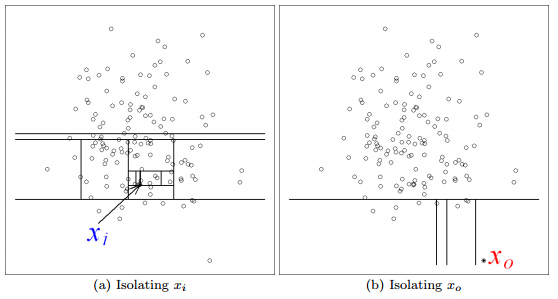
\includegraphics[width=0.8\textwidth]{images/isolation_forest.png}
  \caption[Isolation Forest]{Isolation Forest}%
  \label{fig:hintergrund_isolation_forest}
\end{figure}

Die Pfadlänge wird durch die Anzahl Knoten, die vom Root Node bis zum Ende durchlaufen werden müssen, bestimmt. Da die Partitionsgrenzen zufällig gewählt werden, führt man diese Isolation mehrmals für einen Punkt durch und nimmt davon die durchschnittliche Länge. Je kürzer ein Pfad ist, desto eher handelt es sich um einen Ausreisser. Denn dieser konnte schneller isoliert werden. Abbildung \ref{fig:hintergrund_isolation_forest} zeigt die Isolation  eines normalen Beobachtungswert $Xi$, wobei $b$ die Isolation eines Ausreisser $X_0$ darstellt.

% Newpage if not on new page TODO
Der Anomaly Score wird mit Hilfe der nicht erfolgreichen Suche eines Binary Search Tree berechnet. Dabei ist n die Anzahl Knoten, $E(h(x))$ die durchschnittliche Pfadlänge und $c(n)$ die durchschnittliche Kostenfunktion einer nicht erfolgreichen Suche im Binary Search Tree. Die Formel dafür sieht wie folgt aus:

\begin{equation}\label{eq:isolation}
s(x, n) = 2^{-\frac{E(h(x))}{c(n)}}
\end{equation}

Die Funktion $s(x, n)$ gibt immer einen Wert zwischen 0 und 1 zurück. Wobei 1 einem klaren Ausreisser entspricht \cite{isolation_forest_2}.